%%%%%%%%%%%%%%%%%%%%%%%%%%%%%%%%%%%%%%%%%%%%%%%%%%%%%%%%%%%%%%%%%%%%%%%%%%%%%%%
%%%%%%%%%%%%%%%%%%%%%%%%%%%%%%%%%%%%%%%%%%%%%%%%%%%%%%%%%%%%%%%%%%%%%%%%%%%%%%%
%%%%%%%%%%%%%%%%%%%%%%%%%%%%%%%%%%%%%%%%%%%%%%%%%%%%%%%%%%%%%%%%%%%%%%%%%%%%%%%
%%%%%%%%%%%%%%%%%%%%%%%%%%%%%%%%%%%%%%%%%%%%%%%%%%%%%%%%%%%%%%%%%%%%%%%%%%%%%%%
\chapter{Methodology}
\label{ch:approach}
%%%%%%%%%%%%%%%%%%%%%%%%%%%%%%%%%%%%%%%%%%%%%%%%%%%%%%%%%%%%%%%%%%%%%%%%%%%%%%%
%%%%%%%%%%%%%%%%%%%%%%%%%%%%%%%%%%%%%%%%%%%%%%%%%%%%%%%%%%%%%%%%%%%%%%%%%%%%%%%
%%%%%%%%%%%%%%%%%%%%%%%%%%%%%%%%%%%%%%%%%%%%%%%%%%%%%%%%%%%%%%%%%%%%%%%%%%%%%%%
%%%%%%%%%%%%%%%%%%%%%%%%%%%%%%%%%%%%%%%%%%%%%%%%%%%%%%%%%%%%%%%%%%%%%%%%%%%%%%%

This chapter describes the workflow and implementation I applied to reach my research goals. 
In the first section, I describe the given data set and the approach to infer networks.
This first step of network interference, was primarily driven by a combination of an exploratory data analysis and an iterative pipeline development process.
It serves as a prerequisite for network analysis part of this thesis.
The second section explains the methods I used to analyze the resulting networks regarding network properties, communities, and its development.

%%%%%%%%%%%%%%%%%%%%%%%%%%%%%%%%%%%%%%%%%%%%%%%%%%%%%%%%%%%%%%%%%%%%%%%%%%%%%%%
%%%%%%%%%%%%%%%%%%%%%%%%%%%%%%%%%%%%%%%%%%%%%%%%%%%%%%%%%%%%%%%%%%%%%%%%%%%%%%%
% INFERRING NETWORKS APPROACH
\section{Inferring Spatial Proximity Networks}
\label{sec:infNetworks}
%%%%%%%%%%%%%%%%%%%%%%%%%%%%%%%%%%%%%%%%%%%%%%%%%%%%%%%%%%%%%%%%%%%%%%%%%%%%%%%
%%%%%%%%%%%%%%%%%%%%%%%%%%%%%%%%%%%%%%%%%%%%%%%%%%%%%%%%%%%%%%%%%%%%%%%%%%%%%%%
To yield the first set of functional and non-functional requirements concerning the pipeline, I conducted a data analysis of the given tracking data, and a literature review, already mentioned in section~\ref{ch:relatedwork}.
The data analysis supported the forming of a general understanding of the given dataset, its structure, characteristics and estimation of its quality.
The purpose of the review was to get an overview of the common methods and approaches regarding network analysis in this field of research.
Both results are then used to decide for a network type and its definition of nodes and edges.
Furthermore, I inferred specific pipeline parameters and decided for the procedure of network extraction.


This pipeline was developed, tested and then refined in an iterative process.
Accordingly, the results of the evaluation lead to new or changing functional requirements.
The evaluation is conducted by reviewing the pipeline parameters' effects on network properties and checking the validity and quality of the networks by investigating the age of bees in the resulting network.


%%%%%%%%%%%%%%%%%%%%%%%%%%%%%%%%%%%%%%%%%%%%%%%%%%%%%%%%%%%%%%%%%%%%%%%%%%%%%%%
%%%%%%%%%%%%%%%%%%%%%%%%%%%%%%%%%%%%%%%%%%%%%%%%%%%%%%%%%%%%%%%%%%%%%%%%%%%%%%%
%%%%%%%%%%%%%%%%%%%%%%%%%%%%%%%%%%%%%%%%%%%%%%%%%%%%%%%%%%%%%%%%%%%%%%%%%%%%%%%
%%%%%%%%%%%%%%%%%%%%%%%%%%%%%%%%%%%%%%%%%%%%%%%%%%%%%%%%%%%%%%%%%%%%%%%%%%%%%%%
\subsection{Describing the Dataset}
\label{sec:dataset}
%%%%%%%%%%%%%%%%%%%%%%%%%%%%%%%%%%%%%%%%%%%%%%%%%%%%%%%%%%%%%%%%%%%%%%%%%%%%%%%
%%%%%%%%%%%%%%%%%%%%%%%%%%%%%%%%%%%%%%%%%%%%%%%%%%%%%%%%%%%%%%%%%%%%%%%%%%%%%%%
%%%%%%%%%%%%%%%%%%%%%%%%%%%%%%%%%%%%%%%%%%%%%%%%%%%%%%%%%%%%%%%%%%%%%%%%%%%%%%%
%%%%%%%%%%%%%%%%%%%%%%%%%%%%%%%%%%%%%%%%%%%%%%%%%%%%%%%%%%%%%%%%%%%%%%%%%%%%%%%
The dataset derives from high-resolution video files that capture tagged honey bees of one colony in a single frame observation hive.
The bees are uniquely tagged with circular 12-bit markers (figure~\ref{fig:markers}, section~\ref{ch:intro}).
Two cameras per side filmed the complete honeycomb permanently.
Figure~\ref{fig:obssetup} illustrates the camera setup.
The \emph{recording period} lasted nine weeks (63 days), from 19.07.2016 until 19.09.2016, with some interruptions due to maintenance work and technical failures. An overview about the complete recording period is given in figure~\ref{fig:observation-period} in appendix~\ref{ch:appendix}.

All four cameras, each with a resolution of $4000\times3000$ pixel, record $3.5$ frames per second. 
An image analysis pipeline~\cite{wario2015automatic} detects all bees in each frame.
The resulting detection data is stored in a binary file format.
A python library\footnote{The library is called \texttt{bb-binary} and is created by the Biorobotics Lab. It can be found on GitHub: \url{https://github.com/BioroboticsLab/bb_binary}; Last accessed: 2106-02-16, 04:28PM} provides a frame-level access to those binary files.
The size of the dataset is $470$~GB, about $7.5$~GB of binary data per day.

\begin{figure}
    \centering
    \begin{subfigure}[htb]{\textwidth}
	\centering
	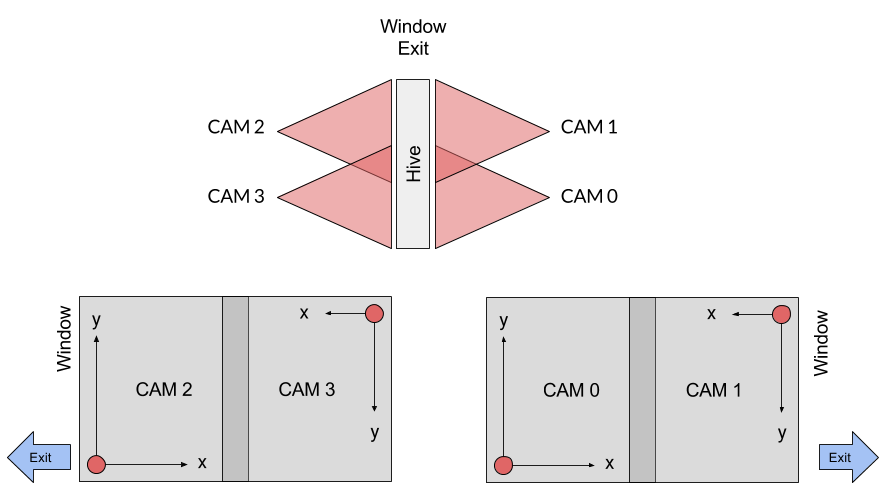
\includegraphics[width=1.0\textwidth]{Figures/setupCams}
	%\caption[Camera setup]{\textbf{Camera setup}}
	%\label{fig:cams}
	\vspace{0mm}
    \end{subfigure}
    \begin{subfigure}[b]{\textwidth}
	\centering
	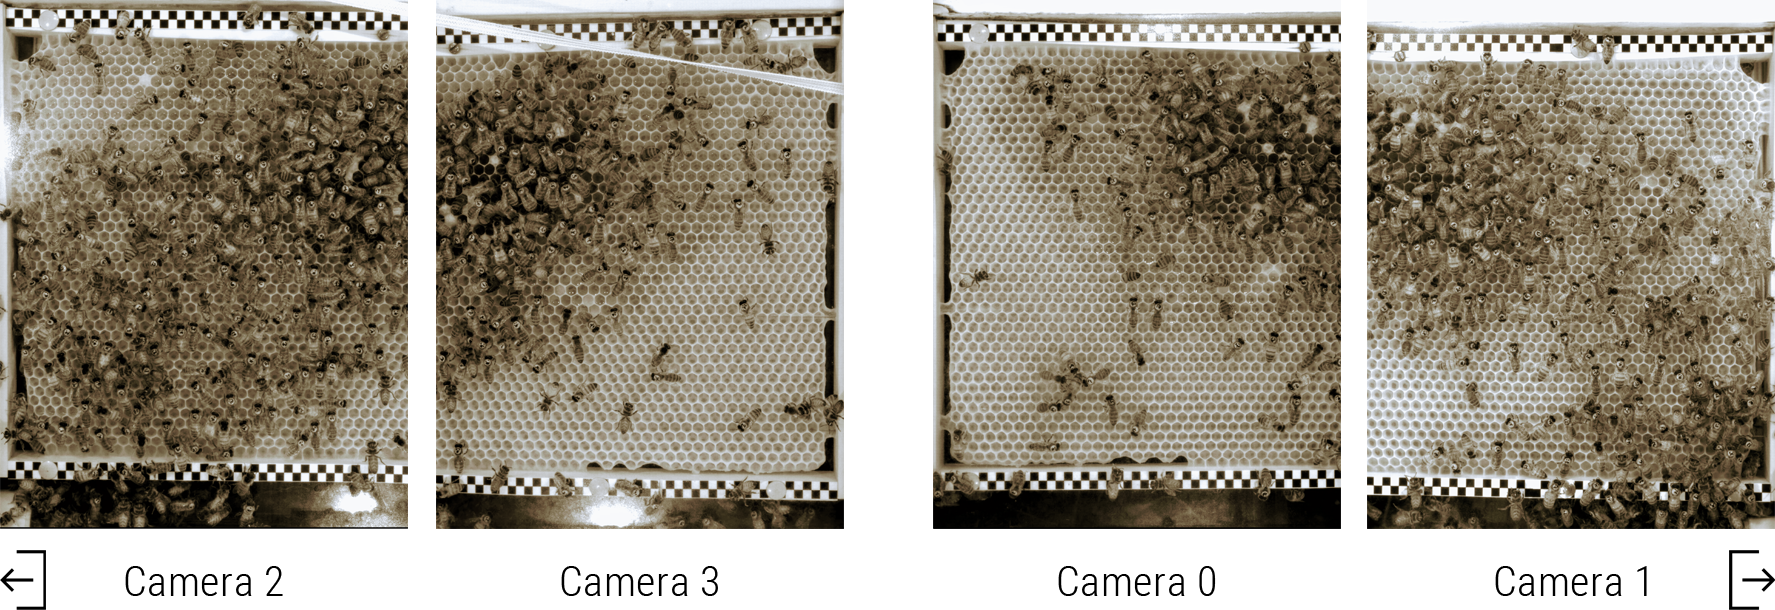
\includegraphics[width=1.0\textwidth]{Figures/beesClose}
    \end{subfigure}
    \vspace{0mm}
 	\caption[Observation setup]{\textbf{Observation setup} Each side of the honeycomb is filmed by two cameras. The two cameras per side overlap, so bees inside this area are detected from both cameras.}
 	\label{fig:obssetup}
\end{figure}

The 67 days long \emph{tagging period} started on 28.06.2016 and lasted until 02.09.2016, resulting in $3.191$ tagged bees. The young bees, which were raised in a separate incubator, were tagged and then added to the observation hive, about noon each day.
Figure~\ref{fig:tagging-period} (Appendix~\ref{ch:appendix}) shows the frequency of tagged bees per day. The hatching day for each bee is documented; therefore the age of each bee at a particular point in time can be calculated.
The life expectancy of a honey bee during summer ranges from 30 to 60 days, according to \textcite[p. 27]{menzel2016intelligenz}
Hence, the maximum number of present bees in the hive is about $1,600$.

For further network analysis, I chose three days: 20., 22., and 24. August.
Those days were chosen because a wide range of age groups was present at this time. The hive especially contained older bees which are likely to be foragers. Besides, no data is missing on those days.


%%%%%%%%%%%%%%%%%%%%%%%%%%%%%%%%%%%%%%%%%%%%%%%%%%%%%%%%%%%%%%%%%%%%%%%%%%%%%%%
%%%%%%%%%%%%%%%%%%%%%%%%%%%%%%%%%%%%%%%%%%%%%%%%%%%%%%%%%%%%%%%%%%%%%%%%%%%%%%%
\subsubsection{Data Scheme}
\label{subsec:datascheme}
%%%%%%%%%%%%%%%%%%%%%%%%%%%%%%%%%%%%%%%%%%%%%%%%%%%%%%%%%%%%%%%%%%%%%%%%%%%%%%%
%%%%%%%%%%%%%%%%%%%%%%%%%%%%%%%%%%%%%%%%%%%%%%%%%%%%%%%%%%%%%%%%%%%%%%%%%%%%%%%

\begin{table}[!t]
\colorbox{usethiscolorhere}{
\centering
\begin{tabularx}{\textwidth}{@{} r Y @{}}
	\textbf{Frame container} &
	Contains all frames, which belong to a specific video file of a certain camera.\\
	\textbf{Frame} &
	Includes all detections of one frame at a certain point in time.\\
	\textbf{Detection} &
	Detection of a bee at a certain point in time.\\
	\textbf{Decoded ID} &
	Identifier of a bee consisting of 12 probability values, representing 12 bits.\\
	\textbf{Confidence} &
	Value between 0\% and 100\%.\\
	\textbf{ID} &
	Decimal representation of a decoded ID.\\
	\textbf{Bee time series} & Binary sequence, indicating the absence and presence of a certain bee in a particular time interval.\\
	\textbf{Pair time series} & Binary sequence, indicating whether or not two bees are close to each other, in a particular time interval.\\
\end{tabularx}
}
\end{table}

The data is organized in so-called \emph{frame containers}.
Each frame container corresponds to one video file of a certain camera and consists of about $1024$ frames.
Each \emph{frame} holds a list of bees, which were detected by the image analysis pipeline.

A bee \emph{detection} has, among others, the following attributes:

\begin{table}[!h]
\centering
\begin{tabular}{rl}
\textbf{xpos}: & $x$ coordinate of bee with respect to the image in pixel \\
\textbf{ypos}: & $y$ coordinate of bee with respect to the image in pixel \\
\textbf{decoded ID}: & decoded 12-bit ID \\
\textbf{cam ID}: & ID of the camera ${0,1,2,3}$ \\
\textbf{timestamp}: & unix timestamp with milliseconds\\
\end{tabular}
\end{table}

The data can be accessed by iterating on the frame level, using a start and end time\-stamp for specifying a time interval. The complete data scheme can be found on GitHub\footnote{\url{https://github.com/BioroboticsLab/bb_binary/blob/master/bb_binary/bb_binary_schema.capnp}; Last accessed: 2106-02-16, 04:46PM}. 


%%%%%%%%%%%%%%%%%%%%%%%%%%%%%%%%%%%%%%%%%%%%%%%%%%%%%%%%%%%%%%%%%%%%%%%%%%%%%%%
%%%%%%%%%%%%%%%%%%%%%%%%%%%%%%%%%%%%%%%%%%%%%%%%%%%%%%%%%%%%%%%%%%%%%%%%%%%%%%%
\subsubsection{ID Probabilities, Confidence Level, and Quality}
\label{subsec:confidence}
%%%%%%%%%%%%%%%%%%%%%%%%%%%%%%%%%%%%%%%%%%%%%%%%%%%%%%%%%%%%%%%%%%%%%%%%%%%%%%%
%%%%%%%%%%%%%%%%%%%%%%%%%%%%%%%%%%%%%%%%%%%%%%%%%%%%%%%%%%%%%%%%%%%%%%%%%%%%%%%

\begin{figure}
    \centering
    \begin{subfigure}[b]{0.45\textwidth}
        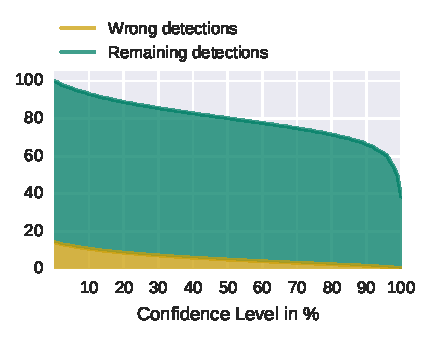
\includegraphics[width=\textwidth]{Figures/detectionsWrongConf}
        \caption[Detections]{\textbf{Detections}}
        \label{fig:detections}
    \end{subfigure}
    \begin{subfigure}[b]{0.45\textwidth}
        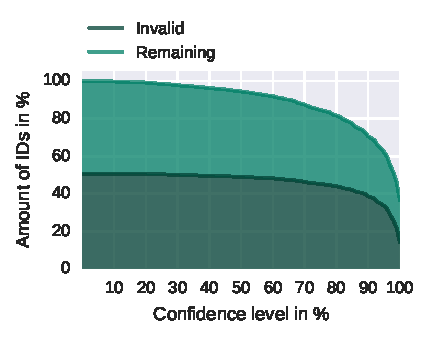
\includegraphics[width=\textwidth]{Figures/idsWrongConf}
        \caption[IDs]{\textbf{IDs}}
        \label{fig:ids}
    \end{subfigure}
 	\caption[Quality of detections and IDs]{\textbf{Quality of detections and IDs} \emph{Light green} represents the number of remaining detections and IDs (from $4096$ possible IDs). \emph{Dark green} indicates the fraction of invalid detections and IDs and in relation to the remaining number of detections and IDs.\protect\footnotemark}
 	\label{fig:remainingVSquality}
\end{figure}

\footnotetext{Data set: 26.07.2016, 4~p.~m., 10~minutes, all cameras}

Twelve bits can encode the identity of 4096 bees.
Each bit of the decoded ID is not a one or zero but represents a probability between $0$ and $255$, normalized to a value between $0$ and $1$.
Therefore, a bit indicates the confidence of the image analysis pipeline for that specific bit.
I define the confidence $c$ for a bit $b$, analogously to Leon~\textcite[p.~14]{leon2016}, as $c(b)=2\cdot|b-0.5|$.
The confidence of a decoded ID is, accordingly, the minimum of all twelve bits' confidences.
Detections with a confidence below a certain level are removed from the data set.
Consequently, a high level of confidence reduces the amount of data, which remains for further processing.

I use the age information of the bees to check the quality of the remaining data.
A bee has a negative age, if the pipeline detected a code, that was not used yet.
I examined the number of remaining bee detections and IDs, depending on the chosen confidence by calculating the age of each bee detection and ID.
A bee detection with a negative age is counted as an \emph{invalid detection}. Also, an ID with a negative age is counted as an \emph{invalid ID}.

As expected, with increasing confidence, the number of remaining detections and IDs decreases (figure~\ref{fig:remainingVSquality}), as well as the fraction of invalid detections and IDs.
With a confidence level of 100\%, the fraction of invalid detections reaches the value of 2.5\%. However, the fraction of invalid IDs stays at the high value of 30.2\%. Consequently, selecting a high level of confidence is not sufficient for obtaining a high data quality.
Therefore, to obtain a more reliable dataset, invalid detections need to be filtered out, in addition to choosing a good level of confidence.

%%%%%%%%%%%%%%%%%%%%%%%%%%%%%%%%%%%%%%%%%%%%%%%%%%%%%%%%%%%%%%%%%%%%%%%%%%%%%%%
%%%%%%%%%%%%%%%%%%%%%%%%%%%%%%%%%%%%%%%%%%%%%%%%%%%%%%%%%%%%%%%%%%%%%%%%%%%%%%%
\subsubsection{Detection Frequency Filter}
\label{subsubsec:dataset:filter}
%%%%%%%%%%%%%%%%%%%%%%%%%%%%%%%%%%%%%%%%%%%%%%%%%%%%%%%%%%%%%%%%%%%%%%%%%%%%%%%
%%%%%%%%%%%%%%%%%%%%%%%%%%%%%%%%%%%%%%%%%%%%%%%%%%%%%%%%%%%%%%%%%%%%%%%%%%%%%%%
\begin{figure}[t]
	\centering
	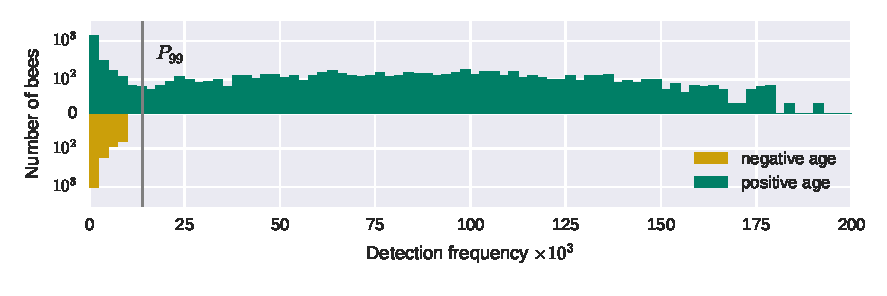
\includegraphics[width=1.0\textwidth]{Figures/filter}
	\caption[Detection frequency of IDs]{\textbf{Detection frequency of IDs} [TODO: add legend] \emph{Orange} coressponds to bees with a negative age and \emph{green} displays bees with a positive age.\protect\footnotemark}
	\label{fig:filter}
\end{figure}
\footnotetext{Data set: 20.08.2016, 24 hours, number of total frames: 302400}

A good indicator, whether a bee detection represents a real bee on the comb is its detection frequency.
The hypothesis is:
Individuals with a very low detection rate seem to be detection errors and lead to the assumption that those bees do not exist.
To check this hypothesis, I investigate the correlation between the detection frequency of bees and their age.
Figure~\ref{fig:filter} shows that bees with a negative age are on average less detected than bees with a positive age.

During my analysis, I noticed the existence of bees with a high detection frequency attributed with a negative age. I inspected the corresponding photos and confirmed that those bee detections correspond to living individuals and are no artifacts. Probably this result from a mistake in the table, which reports the hatching days for each bee.
Consequently, I excluded bees from this analysis, which had a negative age, but a detection frequency over 10,000 frames. Also I excluded bees~($n=10$), whose age is unknown\footnote{id= [2,
    74,
    2045,
    3172,
    3764,
    3796,
    3827,
    3836,
    3844,
    3940]}.
For each analysis day, the number of detections per ID is calculated, excluding the mentioned IDs.
To obtain a reliable dataset, I filtered invalid detections, by discarding all detections with an ID frequency below the 99th percentile of negative IDs.


%%%%%%%%%%%%%%%%%%%%%%%%%%%%%%%%%%%%%%%%%%%%%%%%%%%%%%%%%%%%%%%%%%%%%%%%%%%%%%%
%%%%%%%%%%%%%%%%%%%%%%%%%%%%%%%%%%%%%%%%%%%%%%%%%%%%%%%%%%%%%%%%%%%%%%%%%%%%%%%
\subsubsection{Time Series of Bees and Bee Pairs}
\label{subsec:tracking}
%%%%%%%%%%%%%%%%%%%%%%%%%%%%%%%%%%%%%%%%%%%%%%%%%%%%%%%%%%%%%%%%%%%%%%%%%%%%%%%
%%%%%%%%%%%%%%%%%%%%%%%%%%%%%%%%%%%%%%%%%%%%%%%%%%%%%%%%%%%%%%%%%%%%%%%%%%%%%%%
I investigated the quality of the initial data regarding its completeness of bee tracks. A bee tracks represent the movement of an individual over time. I transformed the initial data set into binary \emph{bee time series}, depicted in figure~\ref{fig:structure} left and middle.
A bee time series, similar to a track, represents the absence and presence of a bee over a specified sequence of frames.
For further processing I use the bee time series to extract \emph{pair time series} of bees that are spatially close (figure~\ref{fig:structure}, right).
A one indicates that a pair of bees is detected and both bees are spatially close in a certain frame.


By analyzing the resulting pair time series, I noticed that the sequences of ones are often interrupted by short sequences of zeroes.
As stated before, the higher the level of confidence, the more data is discarded. This data reduction leads consequently to more zeroes in both time series.
I assume that those short gaps do not refer to any meaningful behavior of the bees. Bees are not able to approach each other and move apart within a second because they simply do not move that fast.
Therefore I concluded, that those gaps originate from detection errors and consequently need to be treated in an appropriate way during further data processing.

\begin{figure}[htb]
	\centering
	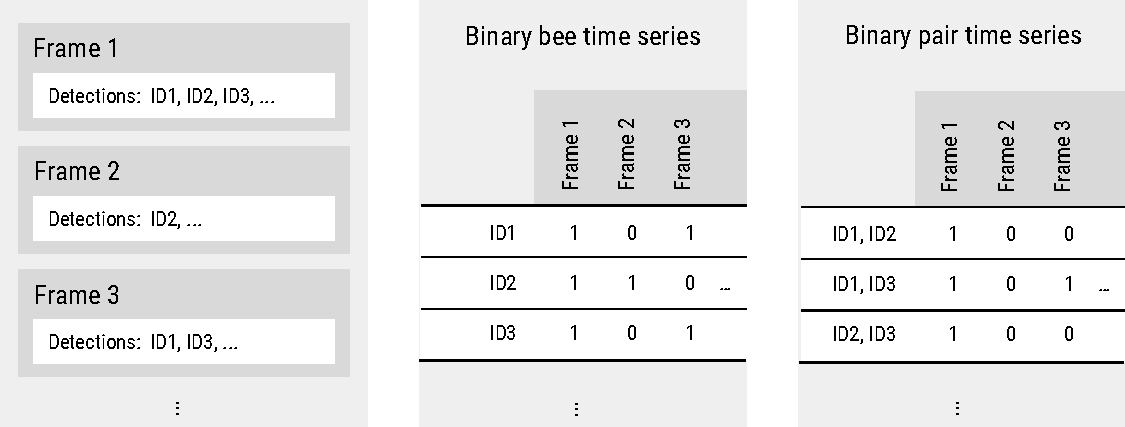
\includegraphics[width=1.0\textwidth]{Figures/structure}
	\caption[Structure of dataset]{\textbf{Structure of dataset} \emph{Left}: original dataset - containing a sequence of frames with bee detections; \emph{Middle:} binary bee time series - zero and one indicate absence and presence of a bee; \emph{Right:} binary pairs time series - zero and one indicate the absence and presence of two bees in the same frame.}
	\label{fig:structure}
\end{figure}


%%%%%%%%%%%%%%%%%%%%%%%%%%%%%%%%%%%%%%%%%%%%%%%%%%%%%%%%%%%%%%%%%%%%%%%%%%%%%%%
%%%%%%%%%%%%%%%%%%%%%%%%%%%%%%%%%%%%%%%%%%%%%%%%%%%%%%%%%%%%%%%%%%%%%%%%%%%%%%%
\subsubsection{Implications}
%%%%%%%%%%%%%%%%%%%%%%%%%%%%%%%%%%%%%%%%%%%%%%%%%%%%%%%%%%%%%%%%%%%%%%%%%%%%%%%
%%%%%%%%%%%%%%%%%%%%%%%%%%%%%%%%%%%%%%%%%%%%%%%%%%%%%%%%%%%%%%%%%%%%%%%%%%%%%%%
[TODO: redo]\\
The confidence level is set to 95\%.
This a good balance between gaps in the time series and quality of the data and amount of remaining data.
Because bee time series contain a lot of short gaps (mean = 3, 95\% confidence), the inference of edges (bees that are spatially close to each other at the same time), should take this into account.
%%%%%%%%%%%%%%%%%%%%%%%%%%%%%%%%%%%%%%%%%%%%%%%%%%%%%%%%%%%%%%%%%%%%%%%%%%%%%%%
%%%%%%%%%%%%%%%%%%%%%%%%%%%%%%%%%%%%%%%%%%%%%%%%%%%%%%%%%%%%%%%%%%%%%%%%%%%%%%%
\subsection{Specifying the Network and its Parameters}
%%%%%%%%%%%%%%%%%%%%%%%%%%%%%%%%%%%%%%%%%%%%%%%%%%%%%%%%%%%%%%%%%%%%%%%%%%%%%%%
%%%%%%%%%%%%%%%%%%%%%%%%%%%%%%%%%%%%%%%%%%%%%%%%%%%%%%%%%%%%%%%%%%%%%%%%%%%%%%%
As this work constitues the first step towards network analysis using this tracking data I chose to infer time-aggregated spatial proximity network. The Accordingly, the interactions are undirected but weighted.
A node in the network is a bee, identified by an ID.
The network consists only of bees that interact with other bees at least once, during the specified time interval.\\
Two bees are associated (spatially close to each other), if their distance is smaller than a \emph{maximum distance}.
Using only this criterion leads to many interactions, resulting in a very dense network because an interaction could only last for 0.33 seconds.
Therefore, an additional parameter the \emph{minimum contact duration} is introduced.
It specifies the minimum time two bees have to spend close to each other to be called associated.

Edges are assigned two attributes.
The first one is the frequency of contacts, meaning how often they share a close position. The second parameter refers to the total duration of contact, so the total time they spend nearby.

%%%%%%%%%%%%%%%%%%%%%%%%%%%%%%%%%%%%%%%%%%%%%%%%%%%%%%%%%%%%%%%%%%%%%%%%%%%%%%%
\subsubsection{Pipeline Parameters}
%%%%%%%%%%%%%%%%%%%%%%%%%%%%%%%%%%%%%%%%%%%%%%%%%%%%%%%%%%%%%%%%%%%%%%%%%%%%%%%
The network pipeline takes two types of parameters. The first set of parameters defines the resulting network and the exact type of spatial proximity. The second set relates to the given data set. Both parameter types are described below.

\begin{table}[htbp]
\centering
\begin{tabularx}{\textwidth}{@{} r Y @{}}
\textbf{Maximum distance} & level of closeness between to individual bees~(in pixel) \vspace{3mm} \\
\textbf{Minimum} & the number of frames two individuals need to spend close\\
\textbf{Contact duration} &  to each other to count it as an interaction ~(in frames) \vspace{3mm} \\
\textbf{Start timestamp}: & starting point of the network aggregation~(as UTC string) \vspace{3mm} \\
\textbf{Window size}: & size of time window for aggregating the network~(in minutes) \\
\end{tabularx}
\end{table}

\begin{table}[htbp]
\centering
\begin{tabularx}{\textwidth}{@{} r Y @{}}
\textbf{Confidence} & level of confidence, as described in section~\nameref{subsec:confidence}~(in percent) \vspace{3mm}\\
\textbf{Valid IDs} & list of valid ids within a specified time interval, as described in section~\nameref{subsubsec:dataset:filter}~(in CSV file format) \vspace{3mm}\\
\textbf{Gap Size} & for correcting, filling gaps in, the time series of bee pairs~(in frames) \vspace{3mm}\\
\textbf{Number of CPUs} & number of used CPUs for parallelization \vspace{3mm}\\
\textbf{Year} & calculate bee IDs and stitching of camera images according to the observation period~(2015 or 2016)\\
\end{tabularx}
\end{table}

%%%%%%%%%%%%%%%%%%%%%%%%%%%%%%%%%%%%%%%%%%%%%%%%%%%%%%%%%%%%%%%%%%%%%%%%%%%%%%%
\subsubsection{Chosen Parameter Values for Network Analysis}
%%%%%%%%%%%%%%%%%%%%%%%%%%%%%%%%%%%%%%%%%%%%%%%%%%%%%%%%%%%%%%%%%%%%%%%%%%%%%%%

For further network analysis, I chose three days: 20., 22., and 24. August.
Those days were selected because a wide range of age groups was present at this time. The hive especially contained older bees which are likely to be foragers. Besides, no data is missing on those days.
The following values are chosen according to biological constraints and similar to other studies, for better comparability.

I chose the length of a bee body, according to \textcite{baracchi2014socio}, as the maximum distance between two bees (figure~\ref{fig:contactRadius}). The average bee length of $212$px ($\pm 16$px)  was determined by manually measuring the length of all bees ($n=337$) of four camera images using the tool ImageJ\footnote{\url{http://imagej.net/Welcome}; Last accessed:
 22.02.2016}.
The minimum contact duration is set to three frames (one second). This value corresponds to~\textcite{mersch2013tracking}, they as also exclude interactions below one second.
The networks are aggregated for ten hours during daylight; this corresponds to the biological rhythms of bees.

The confidence level confidence is set to $95\%$, to keep about 60\% of the data.
The gap size is set to two frames. This value corresponds to the median gap length in the time series of bee pairs.

\begin{figure}[htb]
	\centering
	\begin{subfigure}[b]{0.45\textwidth}
		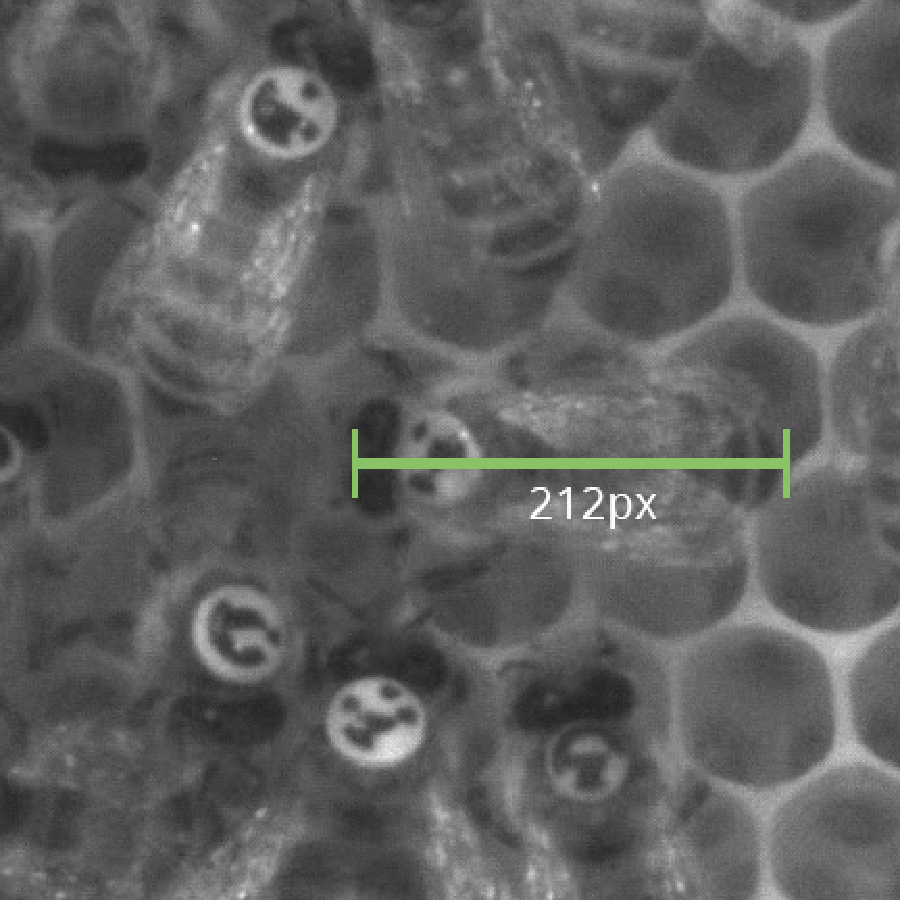
\includegraphics[width=\textwidth]{Figures/sizeTagBee}
		\caption[Body length of a bee]{Body length of a bee}
		\label{fig:size}
	\end{subfigure}
	\hspace{0.08\textwidth}
	\begin{subfigure}[b]{0.45\textwidth}
		\centering
		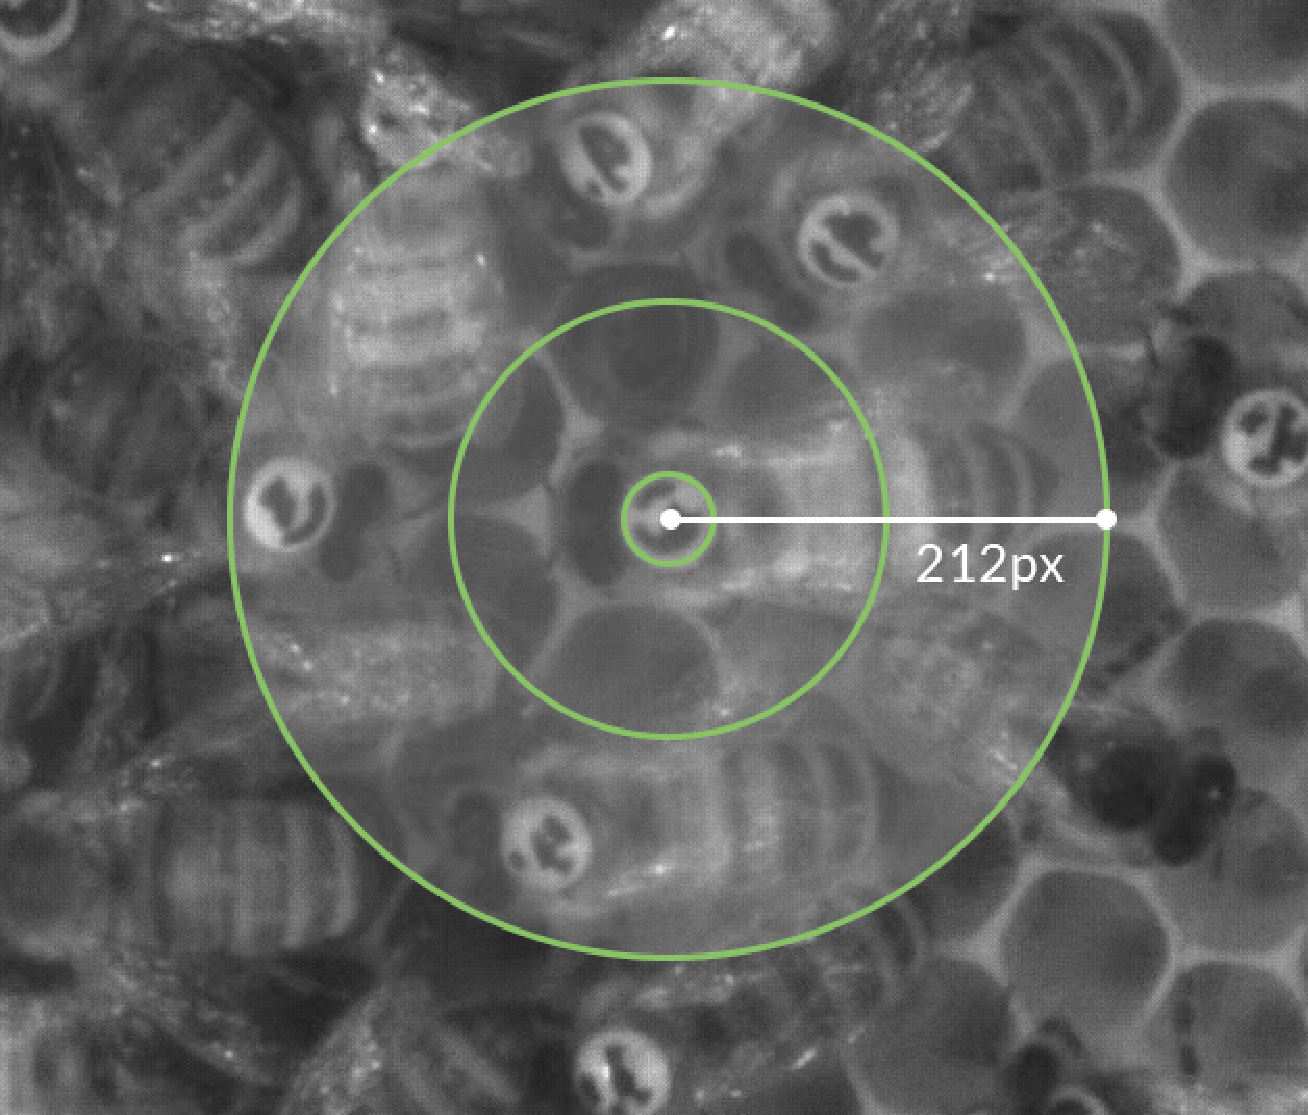
\includegraphics[width=\textwidth]{Figures/radius}
		\caption[Contact radius]{Contact radius}
		\label{fig:radius}
	\end{subfigure}
	\caption[Maximum distance of bees]{\textbf{Maximum distance of bees}: A length of a bee body is chosen as the maximum distance between two bees.}
	\label{fig:contactRadius}
\end{figure}

\begin{table}[htbp]
\small
\centering
\caption[Parameters chosen for network analysis]{\textbf{Parameters chosen for network analysis} The maximum distance corresponds to the length of a bee body and the minimum contact duration is about one second. The networks are aggregated for ten hours.\\
}
\label{tab:chosenparams}

\begin{tabular}{rrl}
	\toprule
	\textbf{Parameter} & \textbf{Value} & \textbf{Unit} \\ \midrule
	Maximum distance & 212 & px \\
	Minimum contact duration & 3 & frames \\
	Window size & 600 & minutes \\ \midrule
	Confidence & 95 & percent \\
	Gap size & 2 & frames \\
	\bottomrule
\end{tabular}

\end{table}
%%%%%%%%%%%%%%%%%%%%%%%%%%%%%%%%%%%%%%%%%%%%%%%%%%%%%%%%%%%%%%%%%%%%%%%%%%%%%%%
%%%%%%%%%%%%%%%%%%%%%%%%%%%%%%%%%%%%%%%%%%%%%%%%%%%%%%%%%%%%%%%%%%%%%%%%%%%%%%%
\subsection{Defining the Network Pipeline}
%%%%%%%%%%%%%%%%%%%%%%%%%%%%%%%%%%%%%%%%%%%%%%%%%%%%%%%%%%%%%%%%%%%%%%%%%%%%%%%
%%%%%%%%%%%%%%%%%%%%%%%%%%%%%%%%%%%%%%%%%%%%%%%%%%%%%%%%%%%%%%%%%%%%%%%%%%%%%%%

This section describes the pipeline for generating spatial proximity networks out of honey bee tracking data. The network pipeline takes as input a path to the data and a set of parameter previously described and outputs a network in graphML file format. I parallelized the pipeline is on the frame level. That means each process gets a fraction of the data and extracts interactions for a time interval of five minutes. The main process accumulates the resulting interactions and creates a final network.

The pipeline consist of the following steps:

\begin{enumerate}
\item \textbf{Prefilter detections}\\
All detections below the chosen level of confidence are filtered out.

\item \textbf{Simple stitching}\\
For each camer positioned on the right hand side of the hive (camera 1 and 3), the $x$-coordinates of each detection is offseted to the right ($2\times \texttt{maximum distance}$), to combine all detections per side into one coordinate system.

\item \textbf{Syncronize cameras}\\
The cameras do not capture all images syncronously and sometime take more or less than $3.5$ images per second.
Therefore, the cameras pers side need to be syncronized. In the normal case the difference between consecutive frames should be about $0.332$~seconds, due to technical problem this value can be lower ($0.003$ ) and higher ($2.932$) at certain times. The frames of cameras 3 and 2 and cameras 1 and 0 are matched, frames without a match are discarded.

\item \textbf{Discard detections with certain IDs}\\
All bee detections with an ID contained in a valid ID list are keept, all other detections are discarded.

\item \textbf{Extract close pairs}\\
For each side of the hive, all close bee pairs according to the maximum distance parameter are calculated using an KDE-tree and then combined.

\item \textbf{Generate time series of bee pairs}\\
The data structure (frames and pairs of bees) is transformed to time series of bee pairs.

\item \textbf{Correct pair time series.}\\
The time series of bees are corrected by filling in the gaps of a certain length (gap size parameter).

\item \textbf{Extract interactions}\\
The edges and its attributes (frequency and duration) are extracted from the time series of bees using the minimum contact duration parameter. A sequence of ones with a length of at least minimum contact duration are evaluated as an interaction . The frequency of those series and the total duration (number of ones) are the attributes.
\end{enumerate}

\subsection{Summary and Results}
[TODO]\\

Networks in general, yes but\\
complex preprocessing of the data essential\\
confidence: reduce amount of data\\
hight confidence: less data, a bit better quality, but more gaps\\
low confidence: a lot of data, bad quality but less gaps\\
stitching cameras: remove duplicates\\
syncronize cameras\\
pre filter detections by ids, whos detection frequency is low\\

Temporal networks, yes but\\
time--aggregated\\
daily networks, because biological useful, other window would be random\\
due to maintainance and technical, camera failures: no period without interruptions\\



% NETWORK ANALYSIS APPROACH
%%%%%%%%%%%%%%%%%%%%%%%%%%%%%%%%%%%%%%%%%%%%%%%%%%%%%%%%%%%%%%%%%%%%%%%%%%%%%%%
%%%%%%%%%%%%%%%%%%%%%%%%%%%%%%%%%%%%%%%%%%%%%%%%%%%%%%%%%%%%%%%%%%%%%%%%%%%%%%%
\section{Methods for Analyzing Spatial Proximity Networks}
%%%%%%%%%%%%%%%%%%%%%%%%%%%%%%%%%%%%%%%%%%%%%%%%%%%%%%%%%%%%%%%%%%%%%%%%%%%%%%%
%%%%%%%%%%%%%%%%%%%%%%%%%%%%%%%%%%%%%%%%%%%%%%%%%%%%%%%%%%%%%%%%%%%%%%%%%%%%%%%
This section outlines the methods I used to investigate the networks on a global, intermediate and local level.
It explains the choice of network measures used for the global analysis.
Also, I report the decision for a community detection algorithm and illustrate the methods to examine the segregation of communities concerning age and spatial distribution.
Furthermore, I explain what approach I used to study the development of communities.

%%%%%%%%%%%%%%%%%%%%%%%%%%%%%%%%%%%%%%%%%%%%%%%%%%%%%%%%%%%%%%%%%%%%%%%%%%%%%%%
\subsection{Investigating the Topology and Network Characteristics}
\label{subsec:APmeasures}
%%%%%%%%%%%%%%%%%%%%%%%%%%%%%%%%%%%%%%%%%%%%%%%%%%%%%%%%%%%%%%%%%%%%%%%%%%%%%%%
I summarized the network analysis methods of the reviewed studies (chapter~\ref{ch:relatedwork}) to gain an overview of established procedures in the field of social insect networks. I grouped the methods by global measures, node level measures and other network analysis methods.
Table~\ref{tab:study-measures} summarizes the used network analysis methods of the reviewed studies.
The network measures I chose for the global and node level analysis are listed in table~\ref{tab:netprop} and were defined in chapter~\ref{sec:definitions}.

The degree of a bee represents the number of other bees this focal animal interacts.
Bees with a high number of interaction partners, have a high degree.
This measure was chosen because it reveals a lot about the general topology of a network.
The strength of a bee is the sum of its edge weights. A high strength refers either to a large number of interaction partners with a low edge weight or a low number of interaction partners with high edge weights. Especially for aggregated networks this measure accumulates valuable information regarding the interaction activity of bees.
The local clustering coefficient (lcc) of a bee indicates how close its interaction partners are to being a clique\footnote{A clique is a complete subgraph.}. A large lcc shows that most of its interaction partners interact with each other. A low lcc indicates the absence of those interactions.
It is a good indicator for the embeddedness of single bees.

The betweenness of a bee measures, how many shortest paths go through that bee. A bee with a high betweenness would be central or important for the network in the sense of information flow. Removing this bee from the hive would lead to the breakdown of information or food flow and would negatively affect the robustness of the network.
The closeness of a bee measures how fast this bee can reach all others in the network. A high closeness would indicate a very short path to every other bee. Regarding information flow, a bee with high closeness can spread e.g. information to all other bees very fast.
I selected these centrality measures exemplarily.

I examined all node level metrics concerning the age of bees and their detection frequency. The global network properties are compared to an Erd\H{o}s-R\'{e}niy  random network, by averaging over 100 runs.

\begin{table}
\small
\centering
\caption[Measures used for analysis]{\textbf{Measures used for analysis} Each measure is explained in chapter~\ref{sec:definitions}}
\vspace*{5mm}
\begin{tabularx}{\textwidth}{p{0.5\linewidth}p{0.5\linewidth}}
\toprule
Global level measures & Node level measures\\
\midrule
Number of nodes $N$ and edges $E$ & Degree $k$ \\
Average degree $\langle k \rangle$ &  Strength $s$\\
Average strength $\langle s \rangle$ &   Local clustering coefficient $c$\\
Density $D$ & Closeness Centrality $C_C$ \\
Diameter $d_{max}$ & Betweenness Centrality $C_B$\\
Number of components & \\
Global clustering coefficient $C_{\Delta}$ &  \\
Average path length $\langle d \rangle$ & \\
Edge weights & \\

\bottomrule
\end{tabularx}
\label{tab:netprop}
\end{table}


%%%%%%%%%%%%%%%%%%%%%%%%%%%%%%%%%%%%%%%%%%%%%%%%%%%%%%%%%%%%%%%%%%%%%%%%%%%%%%%
\subsection{Detecting Communities}
\label{subsec:APcommunityDet}
%%%%%%%%%%%%%%%%%%%%%%%%%%%%%%%%%%%%%%%%%%%%%%%%%%%%%%%%%%%%%%%%%%%%%%%%%%%%%%%
For finding an appropriate community detection algorithms, I checked the reviewed studies for applicable methods and scanned papers, which compare various community detection algorithms. Finally, I checked a subset of algorithms, which I identified as suitable in this context.

The reviewed studies only include two examples of community respectively cluster analysis. \textcite{mersch2013tracking} used the infomap~\cite{rosvall2009map,rosvall2007information} algorithm. According to the authors, this algorithm only works with sparse networks and is therefore not applicable in my case of densely connected spatial proximity networks. \textcite{baracchi2014socio} use a hierarchical clustering to infer groups of bees within the network that are similar regarding the measures strength, eigenvector, and betweenness centrality. In contrast to the resulting groups of community detection, groups identified by hierarchical clustering do not automatically refer to dense subgraphs of the network.

Much literature on the comparative analysis of community detection algorithms exist, e.g.~\cite{yang2016comparative, harenberg2014community}. Some studies seem to be promising, but assume either a power law degree distribution or
evaluate networks with a low density, which is not applicable here.
Thererfore, I tested community detection algorithms implemented in python, to find an algorithm, which works well for my case of animal social networks. The three most common python libraries for network analysis were reviewed: NetworkX\footnote{\url{https://networkx.github.io/}; Last accessed: 16.03.2016, 6:36~p.m.}, igraph\footnote{\url{http://igraph.org/python/}; Last accessed: 16.03.2016, 6:38~p.m.}, and graph-tool\footnote{\url{https://graph-tool.skewed.de/}; Last accessed: 16:03.2016, 6:39~p.m.})
The algorithm needs to fulfill the following criterias:

\begin{itemize}
\item Support for large and very dense networks ($N=1000$, $D>50\%$)
\item Support for weighted edges
\item Fast runtime
\end{itemize}

Table~\ref{tab:algos} gives an overview about the algorithms reviewed. Five algorithms did not terminate after 15~minutes and were therefore excluded from further investigations. Infomap and label propagation tend to partition all nodes into a single community, this is known especially in dense graphs~\cite{yang2016comparative, fortunato2010community}.
The Louvain algorithm~\footnote{Implemented in python for networkX: \url{http://perso.crans.org/aynaud/communities/api.html}} (networkX) is the same as multilevel (iGraph), but takes longer producing almost the same communities and therefore was also excluded. Walktrap was tested for different step size parameters, as suggested in~\cite{pons2005computing}, the communities remained almost the same, only a few nodes switched communities.

I examined the number and size of detected communities for the algorithms fastgreedy, leading eigenvector, multilevel, and walktrap for all three snapshots. Table~\ref{tab:algos4} gives an overview about the results.
All algorithms found at least two communities.
Except for leading eigenvector, most tend to find three communities.

I decided to use two algorithms for community detection: leading eigenvector and walktrap. \textcite{farine2015constructing} explains that leading eigenvector is often used with animal social networks and works well. Walktrap is chosen for also examining the third community.

\begin{table}[htbp]
\small
\caption[Compairing community detection algorithms]{\textbf{Comparing community detection algorithms} Comparison of algorithms implemented in python. Criterias are the support of weighted edges, runtime and number of communities. A runtime indicated by $-$ mean no termination after 15~minutes.\\
}
\label{tab:algos}

\begin{tabularx}{\textwidth}{lcccccccccccc}
\toprule
	 {} &
	 \rotatebox{90}{\textbf{fastgreedy$^1$}} &
	 \rotatebox{90}{\textbf{leading eigenvector$^1$}} &
	 \rotatebox{90}{louvain$^2$} &
	 \rotatebox{90}{\textbf{multilevel$^1$}} &
	 \rotatebox{90}{\textbf{walktrap$^1$}} &
	 
	 \rotatebox{90}{infomap$^1$} &
	 \rotatebox{90}{label propagation$^1$} &
	 
	 \rotatebox{90}{edge betweenness$^1$} &
	 \rotatebox{90}{k-clique communities$^2$\thinspace} &
	 \rotatebox{90}{optimal modularity$^1$} &
	 \rotatebox{90}{spinglass$^1$} &
	 \rotatebox{90}{statistical inference$^3$} \\ \midrule
	 
	 
	 
	 Edge weights & $\times$ & $\times$ & $\times$ & $\times$ & $\times$ & $\times$ & $\times$ & & $\times$ & $\times$ & $\times$ \\ \midrule
	 Runtime in sec & ~$3.6$ & ~$6.3$ & $11.7$ & ~$0.7$ & $19.4$ & $13.2$ & ~$0.2$ & $-$ & $-$ & $-$ & $-$ & $-$ \\ \midrule
	 Communities & $3$ & $2$ & $2$ & $3$ & $2$ & $1$ & $1$ & $-$ & $-$ & $-$ & $-$ & $-$ \\ \midrule
	  & 473 & 488 & 469 & 462 & 490 & 922 &  922 &  &  &  &  &  \\
	  & 434 & 434 & 453 & 427 & 431 &  &  &  &  &  &  &  \\
	  & 15 &  &  & 33 & (1) &  &  &  &  &  &  &  \\
	 \bottomrule
	 
\end{tabularx}
\begin{flushright}
\footnotesize{
$^1$ igraph, $^2$ NetworkX, $^3$ graph-tool\\
}
\end{flushright}

\end{table}

% \hdashline
% \midrule
% \bottomrule
\begin{table}[htbp]
\centering
\caption[X]{\textbf{X} X\\
}
\label{tab:algos4}

\begin{tabular}{lcccc}
\toprule
	 {} &
	 fastgreedy &
	 leading eigenvector &
	 multilevel &
	 walktrap \\ \midrule
	 
	  Network 1
	  & 473 & 488 & 462 & 490 \\
	  & 434 & 434 & 427 & 431 \\
	  & 15 &   & 33 & (1) \\ \midrule
	  Network 2
	  & 504 & 503 & 481 & 372 \\
	  & 467 & 475 & 439 & 311 \\
	  & 7 &   &  58 & 294 \\
	  & & & & (1) \\ \midrule
	  Network 3
	  & 534 & 537 & 505 & 310 \\
	  & 388 & 385 & 415 & 390 \\
	  &  &   &  (2) & 231 \\
	 \bottomrule
	 
\end{tabular}

\end{table}

% \hdashline
% \midrule
% \bottomrule

\subsubsection{Age and Spatial Distribution of Communities}
To answer the question whether communities reflect different age groups, I studied the average age and the general age distribution of communities. I also investigated whether the age division persists in each snapshot. A two-sample Kolmogorov-Smirnov test was used to determine the statistical difference of the age distribution between communities.

To investigate whether communities reflect groups of bees working in different areas of the comb, I used heat maps to determine the core regions per group and snapshot visually.
I stored the positions of all bees present within the ten hour time windows in an SQLite database to faster access the data and to eliminate the time-consuming parsing.

%%%%%%%%%%%%%%%%%%%%%%%%%%%%%%%%%%%%%%%%%%%%%%%%%%%%%%%%%%%%%%%%%%%%%%%%%%%%%%%
\subsection{Development of Community Members}
\label{sec:bg:tracking}
%%%%%%%%%%%%%%%%%%%%%%%%%%%%%%%%%%%%%%%%%%%%%%%%%%%%%%%%%%%%%%%%%%%%%%%%%%%%%%%
According to \textcite{aynaud2013communities} and  \textcite{brodka2014community} there are three main approaches for community detection in temporal networks (sometimes referred to as community tracking): (1) using a static community detection algorithm on several snapshots and then solving a matching problem, (2) using algorithms that are directly suited for temporal networks and (3) using incremental or online algorithms when processing data streams. For each of the three approaches, several methods already exist.
As community tracking is not the main focus of this work, I chose to apply the most natural method out of approach (1): detecting static communities for each snapshot and then matching those communities using set theory.

Two communities at successive time steps are matched if they share enough nodes.
The \emph{match value} between two communities $C$ and $D$ according to \textcite{hopcroft2004tracking} is defined as:

\begin{equation}
\label{eq:match}
\texttt{match}(C,D) = \texttt{min}\left( \frac{\textbar C\cap D \textbar}{\textbar C\textbar }, \frac{\textbar C\cap D \textbar}{\textbar D \textbar }\right)
\end{equation}

This value is between 0 and 1. A high match value occurs when two communities share many nodes and are of a similar size. Communities with the highest value are matched, respectively represent the same community to different points in time. The author suggests applying a threshold to more precisely define what ``share enough nodes'' means. Otherwise, a matching could occur between communities with only 0.1\% of overlapping nodes.

To investigate the total number of bees, that remain in the network over the three snapshots, I inspected the match value of bees in consecutive snapshots. Also, I calculated all match values between communities in consecutive snapshots and additionally calculated the number of intersecting bees. I visualize the dynamic movement
of bees between groups of different snapshots with a flowchart diagram using the JavaScript library D3.js\footnote{\url{https://d3js.org/}}.